\begin{figure}[!t]
\centering
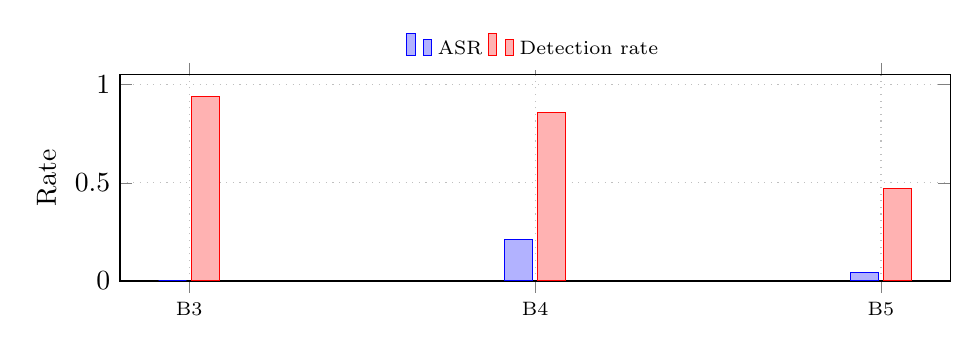
\begin{tikzpicture}
\begin{axis}[
  ybar,
  bar width=10pt,
  width=\columnwidth,
  height=4.2cm,
  ylabel={Rate},
  ymin=0, ymax=1.05,
  symbolic x coords={B3,B4,B5},
  xtick=data,
  xticklabel style={font=\scriptsize},
  legend style={font=\scriptsize, at={(0.5,1.02)}, anchor=south, legend columns=2, draw=none},
  grid=major,
  major grid style={dotted,gray!50},
]
\addplot coordinates {(B3,0.000) (B4,0.211) (B5,0.044)};
\addplot coordinates {(B3,0.939) (B4,0.856) (B5,0.472)};
\legend{ASR, Detection rate}
\end{axis}
\end{tikzpicture}
\caption{Hybrid LLM baselines B3--B5 (6-seed means; CI95 in Table~\ref{tab:llm}). B4 has the highest mean ASR; B5 remains low ($0.044{\pm}0.028$).}
\label{fig:hybrid-asr}
\end{figure}
